\documentclass[a4paper,11pt,fleqn]{article}%fleqn pour aligner les equations à gauche
\usepackage{../../Styles/Cours}

\newcommand{\chnum}{Chapitre 18}
\newcommand{\chtitle}{Diffraction d'une onde lumineuse}
\newcommand{\dtype}{TP}

\begin{document}
\maketitle

La diffraction est utilisée comme technique d'analyse dans l'industrie pour contrôler la taille de petits objets (grains de ciments, de toner d'imprimante, de farine, fils ...)\\
Dans cette activité expérimentale, on observera d'abord les figures de diffraction obtenues avec différents objets diffractants. On exploitera ensuite le phénomène de diffraction afin de déterminer le diamètre d'un cheveu.\\
\noindent
\begin{minipage}[t]{.44\textwidth}
\begin{materiel}
\begin{itemize*}
    \item un laser route (attention aux yeux)
    \item différentes diapositives (vide, avec fente, avec trou)
    \item des fils de diamètres connus : \SI{90}{\micro\meter}, \SI{100}{\micro\meter}, \SI{160}{\micro\meter}, \SI{260}{\micro\meter}, \SI{300}{\micro\meter}
    \item un écran (plaque opaque)
    \item des potences et pinces de fixation
    \item un mètre ruban
    \item du ruban adhésif
    \item un ordinateur muni du logiciel de traitement de données \textit{Latis Pro}
\end{itemize*}
\end{materiel}
\end{minipage}
\begin{minipage}[t]{.55\textwidth}
\begin{documentboxenv}{Figure de diffraction}
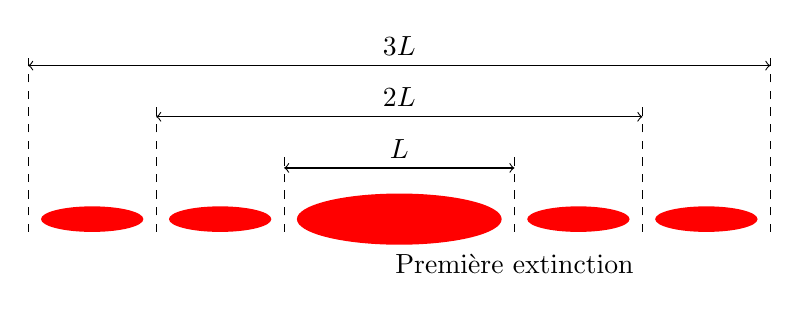
\begin{tikzpicture} [scale=.65]
\fill [red] (0,0) ellipse(2 and .5);
\fill [red] (-3.5,0) ellipse(1 and .25);
\fill [red] (3.5,0) ellipse(1 and .25);
\fill [red] (-6,0) ellipse(1 and .25);
\fill [red] (6,0) ellipse(1 and .25);

\draw [dashed] (-2.25,-0.25) -- (-2.25,1.25);
\draw [dashed] (2.25,-0.25) -- (2.25,1.25);

\draw [dashed] (-2.25,-0.25) -- (-2.25,1.25);
\draw [dashed] (2.25,-0.25) -- (2.25,1.25);

\draw [dashed] (-4.75,-0.25) -- (-4.75,2.25);
\draw [dashed] (4.75,-0.25) -- (4.75,2.25);

\draw [dashed] (-7.25,-0.25) -- (-7.25,3.25);
\draw [dashed] (7.25,-0.25) -- (7.25,3.25);

\draw [<->] (-2.25,1) to (2.25,1);
\draw [<->] (-4.75,2) to (4.75,2);
\draw [<->] (-7.25,3) to (7.25,3);

\draw (0,1) node[above]{$L$};
\draw (0,2) node[above]{$2L$};
\draw (0,3) node[above]{$3L$};

\draw (2.25,-0.5) node[below]{Première extinction};
\end{tikzpicture}
\end{documentboxenv}
\begin{documentboxenv}{Trigonométrie}
Lorsqu'un angle est faible, on peut faire l'approximation suivante : $\tan{\theta} \approx \theta$\\
Exemple : pour $\theta$ = 0,1 \unit{\radian} ($\approx$ 5 \unit{\degree}), $\tan{\theta} \approx$ \num{0,10033} $\approx \theta$  
\end{documentboxenv}
\end{minipage}

\vspace{1em}

\noindent\begin{minipage}{\linewidth}
\begin{documentboxenv}{Incertitude}
De nombreuses sources d'erreurs viennent entâcher la précidion d'une valeur mesurée :
\begin{itemize*}
    \item erreur liée à la source de l'instrumentt utilisé
    \item erreur liée à un facteur etérieur (ex : variations de température)
    \item erreur liée à la lecture du résultat par l'expérimentateur (ex: appréciation de la netteté de l'image)
    \item erreur liée au protocole ou aux manipulations (exemple : pertes de gouttes lors du versage d'un liquide)
\end{itemize*}
Toutes ces erreurs s'accumulent, il faut en tenir compte pour estimer raisonnablement l'incertitude-type.\\
Dans le cas d'une double lecture sur une échelle graduée, l'incertitude-type peut être prisé égale à :
$$ u(X) = \dfrac{1 \text{ graduation}}{\sqrt{6}} $$
\end{documentboxenv}
\end{minipage}

\section{Étude qualitative des figures de diffraction (\emph{durée estimée : 10 min})}
\begin{enumerate}
    \item Braquer un laser rouge vers une fente verticale
    \item Intercaler sur le trajet du rayon laser une fente verticale
    \item Observer la figure de diffraction obtenue puis la représenter dans le tableau ci-dessous.
\end{enumerate}
    \begin{center}
        \begin{tabular}{|>{\centering}m{.17\linewidth}|>{\centering}m{.18\linewidth}|>{\centering}m{.18\linewidth}|>{\centering}m{.17\linewidth}|>{\centering\arraybackslash}m{.17\linewidth}|}
       \hline \textbf{Objet diffractant} & Fente verticale & Fente horizontale & Trou circulaire & Fil vertical\\
        \hline \textbf{Figure de diffraction}&&&&\rule[2cm]{0cm}{0cm}\\
        \hline
    \end{tabular}
    \end{center}
\begin{enumerate}[resume]
    \item Compléter le reste du tableau en recommençant l'expérience avec les autres objets diffractants proposés
    \item Expliquer la forme de la tache de diffraction obtenue avec le trou circulaire
\end{enumerate}

\section{Détermination du diamètre d'un cheveu}
    \subsection{Première méthode (\emph{durée estimée : 40 min})}
    \begin{enumerate}[resume]
        \item Réaliserle montage suivant en utilisant un cheveu à la place de la fente (utiliser la diapositive vide pour fixer le cheveu.
        \begin{center}
            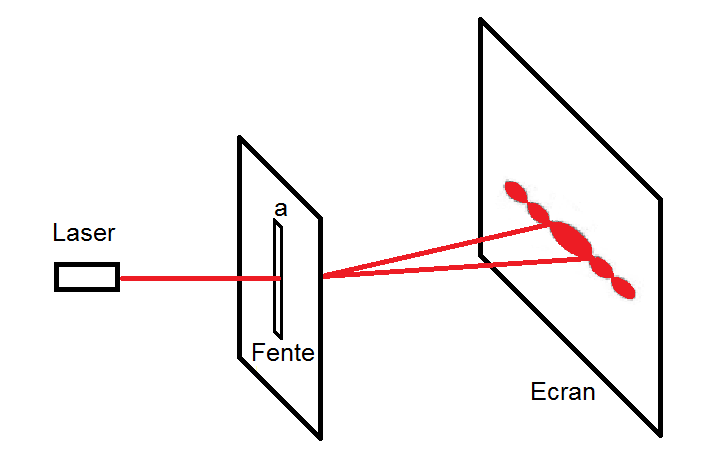
\includegraphics[scale = .5]{Ressources/TSPE_C9_AE1_Fig1.png}
        \end{center}
        \item Faire figurer sur le schéma le diamètre $d$ du cheveu, la distance $D$ entre le cheveu et l'écran et la largeur $L$ de la tache centrale de diffraction
        \item Indiquer quel paramètre expérimental il est possible de modifier pour observer des taches de diffraction les plus grandes possibles. Se placer dans ces conditions.
        \item Justifier que l'angle de diffraction $\theta$ est faible, puis exprimer $\theta$ en fonction de $L$ et $D$.
        \item en déduire une relation entre $d$, $\lambda$, $L$ et $D$.
        \item Mesurer la largeur $L$ de la tache centrale, puis déterminer le diamètre$d$ du cheveu.
    \end{enumerate}
    L'incertitude-type sur le diamètre $d$ du cheveu se détermine à partir de la relation suivante :
        $$ \dfrac{u(d)}{d} = \sqrt{\left( \dfrac{u(L)}{L}\right)^2 +\left( \dfrac{u(D)}{D}\right)^2 + \left( \dfrac{u(\lambda)}{\lambda}\right)^2}$$
    \begin{enumerate}[resume]
        \item Estimer les incertitude-type sur $L$ et $D$. L'incertitude-type sur la longueur d'onde $u(\lambda)$ est considérée comme négligeable par rapport à $u(L)$ et $u(D)$.
        \item Calculer l'incertitude-type $u(d)$ sur le diamètre du cheveu.
        \item Donner le diamètre du cheveu avec son incertitude.
        \item Proposer au moins un moyen de diminuer cette incertitude.
    \end{enumerate}

    \subsection{Deuxième méthode (\emph{durée estimée : 1h})}
    \begin{enumerate}[resume]
        \item À l'aide de la question 10, exprimer $L$ en fonction de $1/d$.
        \item Proposer alors une méthode utilisant le matériel disponible pour déterminer la taille du cheveu.
        \item Mettre en \oe uvre la méthode proposée.
    \end{enumerate}
\end{document}